\section{Exercise two}

Consider the ARMAX system: 
\[y(t)=\dfrac{1}{2}y(t-1)+u(t-1)+e(t)+\dfrac{1}{3}e(t-1)\qquad e(t)\sim WN(0,1)\]
\begin{enumerate}
    \item Check the assumptions for designing a Minimum Variance Controller.
    \item Compute the one-step ahead predictor.
    \item Compute the Minimum Variance Controller.
    \item Draw the closed-loop schema.
    \item Find the transfer function from $y^0(t)$ to $y(t)$.
    \item Find the transfer function from $e(t)$ to $y(t)$.
    \item Check the closed-loop stability.
\end{enumerate}

\subsection*{Solution}
\begin{enumerate}
    \item The system in canonical form is:
        \[y(t)=\dfrac{1}{1-\frac{1}{2}z^{-1}}u(t-1)+\dfrac{1+\frac{1}{3}z^{-1}}{1-\frac{1}{2}z^{-1}}e(t-1)\]
        The assumptions are:
        \begin{itemize}
            \item $b_0\neq 0$: $b_0=1$, satisfying the condition.
            \item $B(z)$ is minimum phase: both models have no roots, thus minimum phase.
            \item $\frac{C(z)}{A(z)}$ is in canonical form: both models are constructed in canonical form.
            \item We assume that $y^0(t)$ is independent of $e(t)$, and $y^0(t)$ is unpredictable. 
        \end{itemize}
    \item The one-step ahead predictor is given by:
        \[\hat{y}(t|t-1)=\dfrac{B(z)}{C(z)}u(t-k)+\dfrac{C(z)-A(z)}{C(z)}y(t)\]
        In our case, we have:
        \[\hat{y}(t|t-1)=\dfrac{1}{1+\frac{1}{3}z^{-1}}u(t-1)+\dfrac{\frac{5}{6}}{1+\frac{1}{3}z^{-1}}y(t-1)\]
    \item To find the Minimum Variance Control for both systems, we start with the formula:
        \[u(t)=\dfrac{1}{B(z)E(z)}\left(C(z)y^0(t)-\tilde{R}(z)y(t)\right)\]
        In our case, we have:
        \[u_(t)=\left(\left(1+\dfrac{1}{3}z^{-1}\right)y^0(t)-\dfrac{5}{6}y(t)\right)\]

        We can also derive the control formula from the predictor. 
        Starting with:
        \[\hat{y}(t|t-1)=\dfrac{1}{1+\frac{1}{3}z^{-1}}u(t-1)+\dfrac{\frac{5}{6}}{1+\frac{1}{3}z^{-1}}y(t-1)\]
        After shifting one sample, we get:
        \[\hat{y}(t+1|t)=\dfrac{1}{1+\frac{1}{3}z^{-1}}u(t)+\dfrac{\frac{5}{6}}{1+\frac{1}{3}z^{-1}}y(t)\]
        We impose that $\hat{y}(t+k|t)=y^0(t)$: 
        \[y^0(t)=\dfrac{1}{1+\frac{1}{3}z^{-1}}u(t)+\dfrac{\frac{5}{6}}{1+\frac{1}{3}z^{-1}}y(t)\]
        By isolating the the term $y^0(t)$, we obtain:
        \[u_(t)=\left(\left(1+\dfrac{1}{3}z^{-1}\right)y^0(t)-\dfrac{5}{6}y(t)\right)\]
    \item The closed-loop schema is represented by the following diagram:
        \begin{figure}[H]
            \centering
            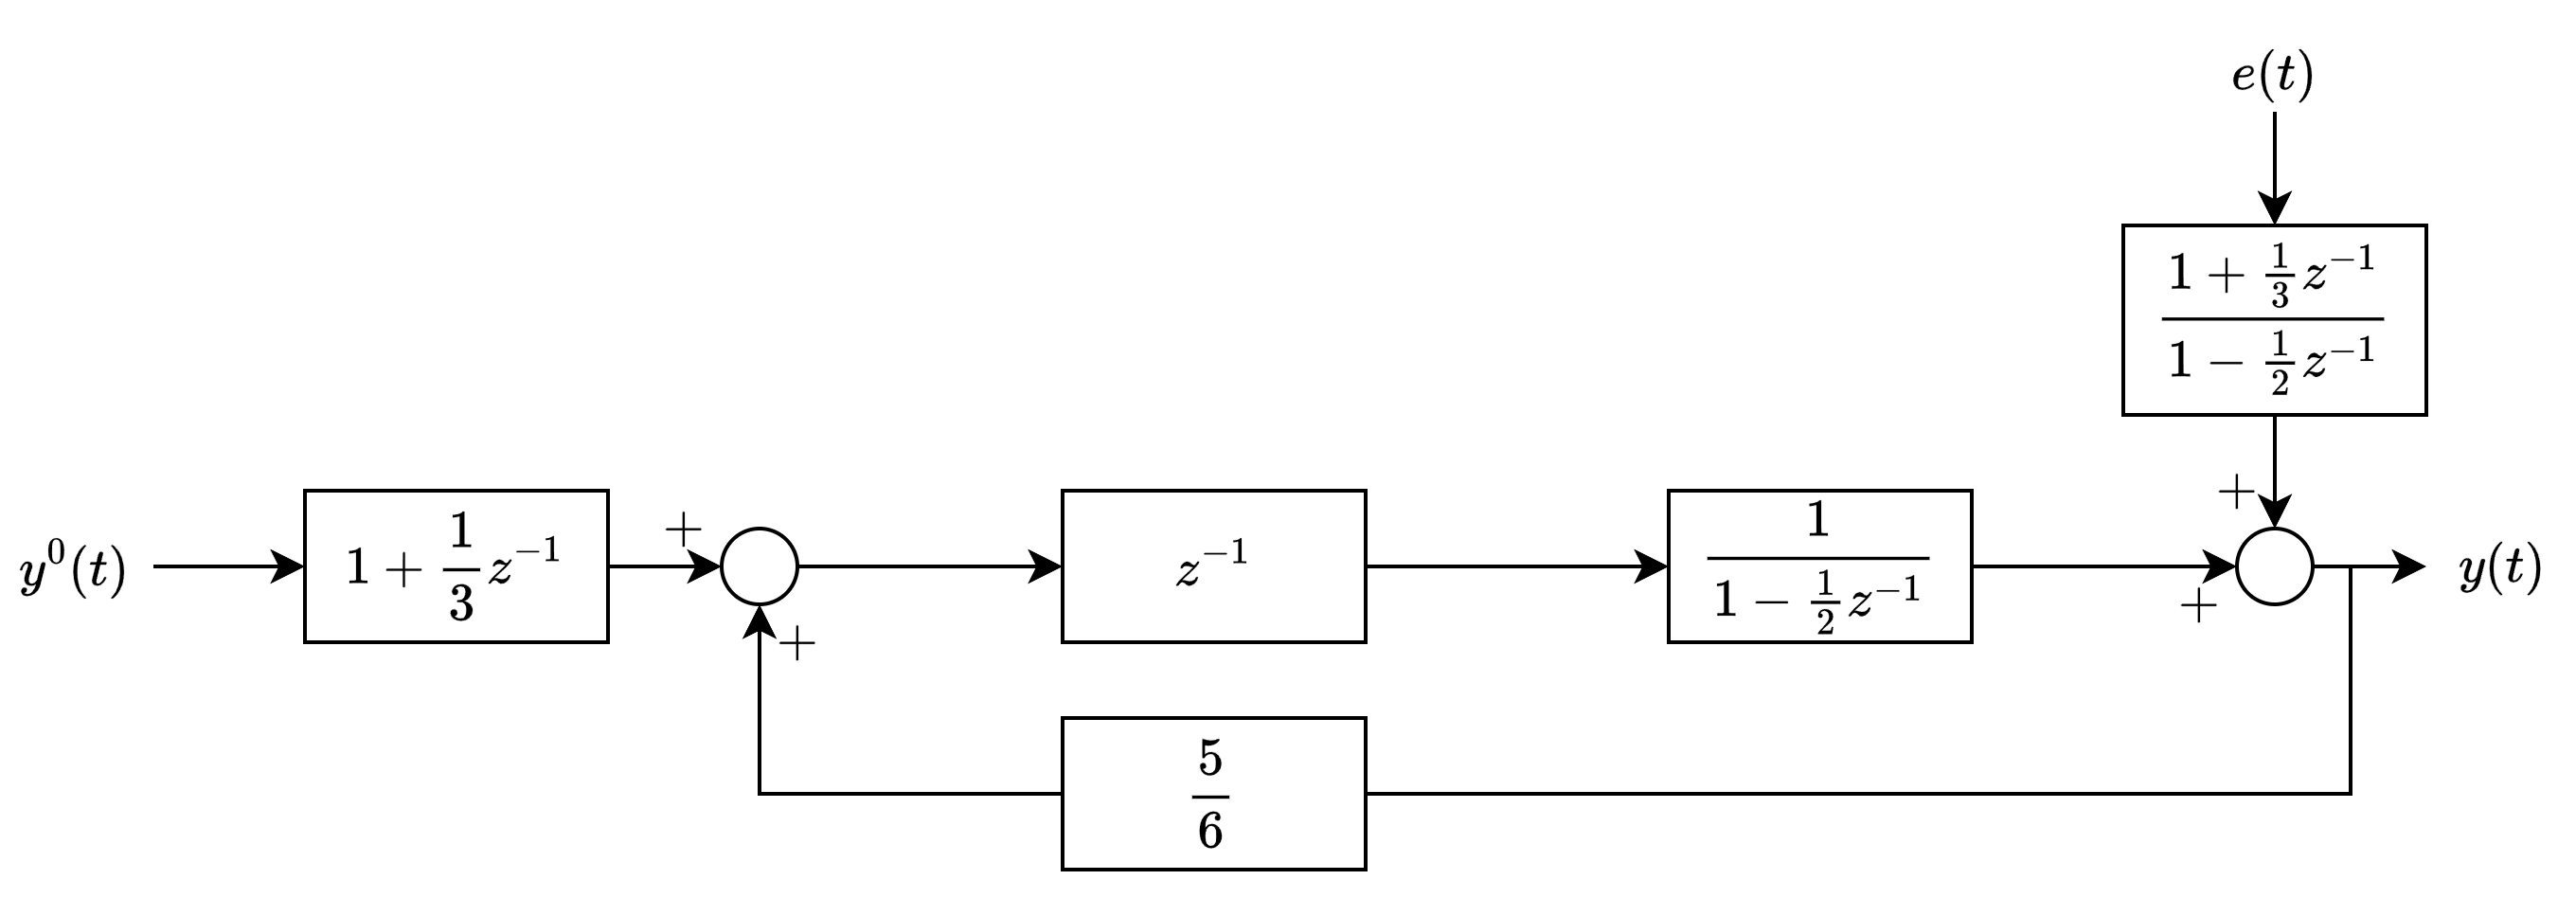
\includegraphics[width=0.75\linewidth]{images/ex2.png}
        \end{figure}
    \item The system equations are given by:
        \[\begin{cases}
            y(t)=\dfrac{1}{1-\frac{1}{2}z^{-1}}u(t-1)+\dfrac{1+\frac{1}{3}z^{-1}}{1-\frac{1}{2}z^{-1}}e(t-1) \\
            u(t)=\left(\left(1+\dfrac{1}{3}z^{-1}\right)y^0(t)-\dfrac{5}{6}y(t)\right)
        \end{cases}\]
        By substituting $u(t)$ into the equation for $y(t)$, we get:
        \[y(t)=\dfrac{1}{1-\frac{1}{2}z^{-1}}z^{-1}\left(\left(1+\dfrac{1}{3}z^{-1}\right)y^0(t)-\dfrac{5}{6}y(t)\right)+\dfrac{1+\frac{1}{3}z^{-1}}{1-\frac{1}{2}z^{-1}}e(t-1)\]
        Isolating the $y(t)$ term, we simplify to:
        \[y(t)=z^{-1}y^0(t)+e(t)\]
    \item From the block scheme, we find that:
        \[W_{ey}=\dfrac{\frac{C(z)}{A(z)}}{1+\frac{1}{B(z)E(z)}z^{-1}\frac{B(z)}{A(z)}\tilde{R}(z)}=E(z)\]
    \item Given that:
        \[\chi(z)=B(z)C(z)=1\left(1+\dfrac{1}{3}z^{-1}\right)=1+\dfrac{1}{3}z^{-1}\]
        we conclude that the system exhibits asymptotic stability because the root lies inside the unit circle.
\end{enumerate}